\documentclass[11pt]{article}
\usepackage[T1]{fontenc}
\usepackage{lmodern}
\usepackage[a4paper,left=25mm,right=30mm,top=22mm,bottom=24mm,marginparwidth=18mm]{geometry}
\usepackage{amsmath,amssymb,mathtools,stmaryrd}
\usepackage{tikz}
\usetikzlibrary{arrows.meta,calc,positioning}
\usepackage{caption}
\usepackage{xcolor}
\usepackage{marginnote}
\usepackage{microtype}
\usepackage{needspace}
\usepackage[hidelinks]{hyperref}
\definecolor{LeanTeal}{HTML}{087F72}
\definecolor{SourceGray}{HTML}{66736F}
\setlength{\parindent}{0pt}
\setlength{\parskip}{0.55em}
\setlength{\emergencystretch}{2em}
\newcommand{\leanmarker}[2]{%
  \Needspace{3\baselineskip}%
  \marginnote{\hyperlink{#1}{\color{LeanTeal}\fbox{\scriptsize Lean}}}%
  \hypertarget{#1}{\textbf{#2.}}%
}
\newcommand{\sourcepage}[1]{\par\medskip\noindent\textcolor{SourceGray}{\scriptsize Source PDF page #1}\par\smallskip}
\pagestyle{plain}
\begin{document}
\begin{center}\LARGE\bfseries Cartesian closed categories of domains\par\medskip
\large Lean 4 Formalization Companion -- Chapter 4\end{center}
\medskip
\noindent\textit{This project-generated reading copy contains reviewed mathematical items, short source locators, and redrawn diagrams. It does not reproduce the original PDF or automatic OCR prose. Click a Lean tag in the web reader to open the mapped Lean declaration.}
\bigskip\hrule\bigskip
\section*{Section 4.0}
\sourcepage{54}
\leanmarker{def-4-0-1}{Definition 4.0.1} Let $D$ and $E$ be dcpos, with $E$ pointed.  For $d\in D$ and $e\in E$, the step function $(d\searrow e):D\to E$ is
\[
(d\searrow e)(x)=
\begin{cases}
e,& x\in \operatorname{Int}(\uparrow d),\\
\bot_E,& \text{otherwise.}
\end{cases}
\]
More generally, $(O\searrow e)$ maps the Scott-open set $O$ to $e$ and maps its complement to $\bot_E$.

\leanmarker{prop-4-0-2}{Proposition 4.0.2}
\begin{enumerate}
\item Step functions are Scott-continuous.
\item If $D,E$ are dcpos, $E$ is pointed, $f:D\to E$ is continuous, and $e\ll f(d)$, then $(d\searrow e)\ll f$.
\item If, in addition, $D$ and $E$ are continuous, then every continuous $f:D\to E$ is a supremum of step functions.
\end{enumerate}
\textit{Proof.} (1) Scott continuity follows because $\operatorname{Int}(\uparrow d)$, and more generally $O$, is Scott-open. (2) Let $G$ be directed and suppose $\bigvee G\sqsupseteq f$. Suprema in $[D\to E]$ are pointwise, so $\bigvee_{g\in G}g(d)\sqsupseteq f(d)$. Since $e\ll f(d)$, some $g\in G$ satisfies $e\sqsubseteq g(d)$; a case split on membership in $\operatorname{Int}(\uparrow d)$ gives $(d\searrow e)\sqsubseteq g$. (3) Given $d\in D$ and $e\ll f(d)$, continuity of $D$ and preservation of directed suprema give
\[
 f(d)=f\!\left(\bigvee_{y\ll d}y\right)=\bigvee_{y\ll d}f(y).
\]
Thus $e\sqsubseteq f(y)$ for some $y\ll d$, and $(y\searrow e)\ll f$ maps $d$ to $e$. Continuity of $E$ supplies such $e$ arbitrarily close to $f(d)$, proving the supremum claim.

\begin{figure}[ht]
\centering
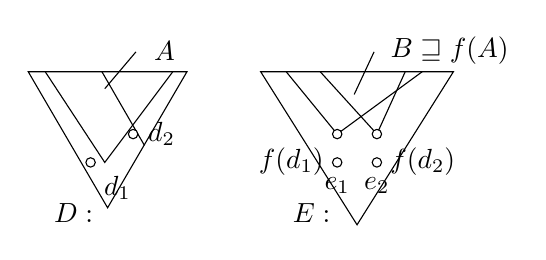
\begin{tikzpicture}[scale=0.72]
  \tikzset{dot/.style={circle,draw,fill=white,inner sep=0pt,minimum size=3.4pt}}
  % D side
  \node at (-3.1,-1.15) {$D:$};
  \draw (-3.9,1.35)--(-1.1,1.35)--(-2.5,-1.05)--cycle;
  \draw (-3.6,1.35)--(-2.55,-0.25)--(-1.35,1.35);
  \draw (-2.6,1.35)--(-1.85,0.05);
  \node[dot,label=below right:{$d_1$}] at (-2.8,-0.25) {};
  \node[dot,label=right:{$d_2$}] at (-2.05,0.25) {};
  \draw (-2.0,1.7)--(-2.55,1.05);
  \node[right] at (-1.85,1.72) {$A$};
  % E side
  \node at (1.1,-1.15) {$E:$};
  \draw (0.2,1.35)--(3.6,1.35)--(1.9,-1.35)--cycle;
  \draw (0.65,1.35)--(1.55,0.25)--(3.05,1.35);
  \draw (1.25,1.35)--(2.25,0.25)--(2.75,1.35);
  \node[dot,label=below left:{$f(d_1)$}] at (1.55,0.25) {};
  \node[dot,label=below right:{$f(d_2)$}] at (2.25,0.25) {};
  \node[dot,label=below:{$e_1$}] at (1.55,-0.25) {};
  \node[dot,label=below:{$e_2$}] at (2.25,-0.25) {};
  \draw (2.2,1.7)--(1.85,0.95);
  \node[right] at (2.32,1.72) {$B\sqsupseteq f(A)$};
\end{tikzpicture}
\caption*{Figure 10: Finding an upper bound for two step functions.}
\end{figure}

\clearpage
\section*{Section 4.1}
\sourcepage{55}
\leanmarker{def-4-1-1}{Definition 4.1.1} Let $E$ be a pointed continuous domain.
\begin{enumerate}
\item $E$ is an $L$-domain if every pair $e_1,e_2\leq e$ has a supremum in $\downarrow e$.
\item $E$ is bounded-complete if every bounded pair has a supremum.
\item $E$ is a continuous lattice if every pair has a supremum.
\end{enumerate}
The corresponding full subcategories are denoted $L$, $BC$, and $LAT$, with algebraic counterparts $aL$, $aBC$, and $aLAT$.

\begin{figure}[ht]
\centering
\setlength{\tabcolsep}{2.2em}
\begin{tabular}{ccc}
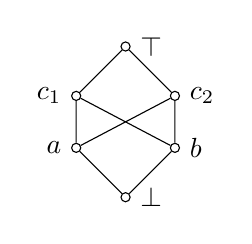
\begin{tikzpicture}[scale=0.66,baseline=(current bounding box.center)]
  \tikzset{dot/.style={circle,draw,fill=white,inner sep=0pt,minimum size=3.3pt}}
  \node[dot,label=right:{$\top$}] (top) at (0,2.3) {};
  \node[dot,label=left:{$c_1$}] (c1) at (-0.95,1.35) {};
  \node[dot,label=right:{$c_2$}] (c2) at (0.95,1.35) {};
  \node[dot,label=left:{$a$}] (a) at (-0.95,0.35) {};
  \node[dot,label=right:{$b$}] (b) at (0.95,0.35) {};
  \node[dot,label=right:{$\bot$}] (bot) at (0,-0.6) {};
  \draw (bot)--(a)--(c1)--(top)--(c2)--(b)--(bot);
  \draw (a)--(c2) (b)--(c1);
\end{tikzpicture}
&
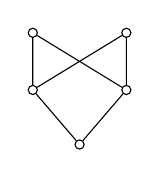
\begin{tikzpicture}[scale=0.66,baseline=(current bounding box.center)]
  \tikzset{dot/.style={circle,draw,fill=white,inner sep=0pt,minimum size=3.3pt}}
  \node[dot] (lt) at (-0.9,1.45) {};
  \node[dot] (rt) at (0.9,1.45) {};
  \node[dot] (lm) at (-0.9,0.35) {};
  \node[dot] (rm) at (0.9,0.35) {};
  \node[dot] (bot) at (0,-0.7) {};
  \draw (bot)--(lm)--(lt);
  \draw (bot)--(rm)--(rt);
  \draw (lm)--(rt) (rm)--(lt);
\end{tikzpicture}
&
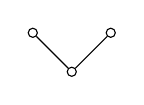
\begin{tikzpicture}[scale=0.66,baseline=(current bounding box.center)]
  \tikzset{dot/.style={circle,draw,fill=white,inner sep=0pt,minimum size=3.3pt}}
  \node[dot] (l) at (-0.75,0.75) {};
  \node[dot] (r) at (0.75,0.75) {};
  \node[dot] (b) at (0,0) {};
  \draw (b)--(l) (b)--(r);
\end{tikzpicture}
\\[-0.1em]
$X\in\mathbf{ALG}\setminus\mathbf L$ & $C\in\mathbf L\setminus\mathbf{BC}$ & $V\in\mathbf{BC}\setminus\mathbf{LAT}$
\end{tabular}
\caption*{Figure 11: Separating examples for the categories of lattice-like domains.}
\end{figure}

\sourcepage{56}
\leanmarker{prop-4-1-2}{Proposition 4.1.2} For a pointed continuous domain $D$, being an $L$-domain, a bc-domain, or a continuous lattice is equivalent respectively to having infima for bounded nonempty subsets, nonempty subsets, or arbitrary subsets.
\textit{Source status.} The textbook states this equivalence without a local proof.

\leanmarker{prop-4-1-3}{Proposition 4.1.3} Retracts and bilimits of $L$-domains, bc-domains, and continuous lattices are again objects of the same respective class.
\textit{Source derivation.} The retract/bilimit part follows from Proposition 3.1.2 and Theorem 3.1.4; preservation of the required infima by upper adjoints gives the lattice-like part.

\sourcepage{57}
\leanmarker{prop-4-1-4}{Proposition 4.1.4} If $D$ is an $L$-domain, a bc-domain, or a continuous lattice, then $\operatorname{Idl}(D,\sqsubseteq)$ is respectively an algebraic $L$-domain, an algebraic bc-domain, or an algebraic lattice.
\textit{Source status.} The textbook states this result without a local proof.

\leanmarker{prop-4-1-5}{Proposition 4.1.5} If $D$ is a continuous domain and $E$ is an $L$-domain, a bc-domain, or a continuous lattice, then the function space $[D\to E]$ is again respectively an $L$-domain, a bc-domain, or a continuous lattice.
\textit{Source status.} The textbook states the closure result here but supplies no local proof.

\leanmarker{cor-4-1-6}{Corollary 4.1.6} The categories $L$, $BC$, $LAT$, and their algebraic counterparts are cartesian closed.
\textit{Source derivation.} This is stated as the consequence of the preceding closure results; no separate proof is printed.

\clearpage
\section*{Section 4.2}
\leanmarker{def-4-2-1}{Definition 4.2.1} Let $P$ be a poset.
\begin{enumerate}
\item $P$ is mub-complete if every upper bound of a finite set $M\subseteq P$ lies above a minimal upper bound of $M$; equivalently,
\[
\bigcap_{m\in M}\uparrow m = \uparrow\operatorname{mub}(M).
\]
\item The mub-closure $\operatorname{mc}(A)$ is the least superset of $A$ closed under adjoining $\operatorname{mub}(M)$ for finite $M$.
\item $P$ has the finite mub property if it is mub-complete and every finite subset has finite mub-closure; with a least element it is a Plotkin order.
\item An algebraic domain whose compact basis is a Plotkin order is called bifinite; the full subcategory of $ALG_\bot$ is denoted $B$.
\end{enumerate}

\sourcepage{58}
\leanmarker{def-4-2-2}{Definition 4.2.2} Let $D$ be bifinite and $E$ pointed algebraic. A finite set $F\subseteq K(D)\times K(E)$ is joinable if
\[
\forall G\subseteq F\;\exists H\subseteq F\;\Bigl(
\pi_1(H)=\operatorname{mub}(\pi_1(G))\ \land\
\forall c\in\pi_2(G)\;\forall d\in\pi_2(H),\ c\sqsubseteq d\Bigr).
\]
The function associated with a joinable family $F$ is
\[
x\longmapsto \bigvee\{e\mid \exists d\in K(D),\ d\sqsubseteq x\ \land\ (d,e)\in F\}.
\]

\leanmarker{lemma-4-2-3}{Lemma 4.2.3} If $D$ is bifinite and $E$ is pointed algebraic, every joinable subset of $K(D)\times K(E)$ gives a compact element of $[D\to E]$. For joinable families $F,G$, the associated functions satisfy the stated order exactly when every $(d,e)\in G$ is matched by some $(d',e')\in F$ with $d'\sqsubseteq d$ and $e\sqsubseteq e'$.
\textit{Source status.} The textbook gives the statement but no proof of the finite-step construction or comparison criterion.

\leanmarker{prop-4-2-4}{Proposition 4.2.4} If $D$ is bifinite and $E$ is pointed algebraic, then $[D\to E]$ is algebraic, and all compact elements of $[D\to E]$ arise from joinable families.
\textit{Proof sketch.} Let \(f:D\to E\) be continuous, let \(M\) be a finite mub-closed set of compact elements of \(D\), and choose compact elements \((e_m)_{m\in M}\) of \(E\) with \(e_m\sqsubseteq f(m)\). One constructs compact elements \((\widehat e_m)_{m\in M}\) so that \(m\mapsto\widehat e_m\) is order-preserving, by repeatedly choosing an upper bound for \(\{e_m\}\cup\{\widehat e_{m'}\mid m'<m\}\). This yields a directed collection of compact elements of \([D\to E]\) arbitrarily close to \(f\).

\begin{figure}[ht]
\centering
\setlength{\tabcolsep}{1.7em}
\begin{tabular}{ccc}
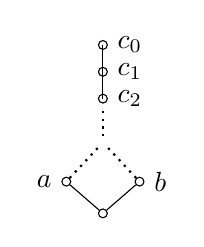
\begin{tikzpicture}[scale=0.62,baseline=(current bounding box.center)]
  \tikzset{dot/.style={circle,draw,fill=white,inner sep=0pt,minimum size=3.2pt}}
  \node[dot,label=right:{$c_0$}] at (0,2.8) {};
  \node[dot,label=right:{$c_1$}] at (0,2.25) {};
  \node[dot,label=right:{$c_2$}] at (0,1.7) {};
  \draw (0,1.7)--(0,2.8);
  \draw[dotted,line width=0.8pt] (0,1.45)--(0,0.85);
  \node[dot,label=left:{$a$}] (a) at (-0.75,0.0) {};
  \node[dot,label=right:{$b$}] (b) at (0.75,0.0) {};
  \node[dot] (bot) at (0,-0.65) {};
  \draw (bot)--(a) (bot)--(b);
  \draw[dotted,line width=0.8pt] (a)--(-0.05,0.75) (b)--(0.05,0.75);
\end{tikzpicture}
&
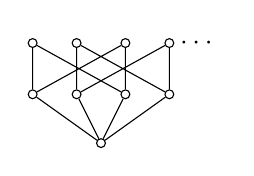
\begin{tikzpicture}[scale=0.62,baseline=(current bounding box.center)]
  \tikzset{dot/.style={circle,draw,fill=white,inner sep=0pt,minimum size=3.2pt}}
  \node[dot] (bot) at (0,-0.8) {};
  \foreach \i/\x in {1/-1.4,2/-0.5,3/0.5,4/1.4} {
    \node[dot] (l\i) at (\x,0.2) {};
    \node[dot] (u\i) at (\x,1.25) {};
    \draw (bot)--(l\i)--(u\i);
  }
  \draw (l1)--(u3) (l2)--(u4) (l3)--(u1) (l4)--(u2);
  \node at (2.0,1.25) {$\cdots$};
\end{tikzpicture}
&
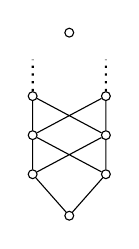
\begin{tikzpicture}[scale=0.62,baseline=(current bounding box.center)]
  \tikzset{dot/.style={circle,draw,fill=white,inner sep=0pt,minimum size=3.2pt}}
  \node[dot] (top) at (0,3.0) {};
  \node[dot] (l3) at (-0.75,1.7) {};
  \node[dot] (r3) at (0.75,1.7) {};
  \node[dot] (l2) at (-0.75,0.9) {};
  \node[dot] (r2) at (0.75,0.9) {};
  \node[dot] (l1) at (-0.75,0.1) {};
  \node[dot] (r1) at (0.75,0.1) {};
  \node[dot] (bot) at (0,-0.75) {};
  \draw (bot)--(l1)--(l2)--(l3);
  \draw (bot)--(r1)--(r2)--(r3);
  \draw (l1)--(r2) (r1)--(l2) (l2)--(r3) (r2)--(l3);
  \draw[dotted,line width=0.8pt] (l3)--(-0.75,2.45) (r3)--(0.75,2.45);
\end{tikzpicture}
\\[-0.1em]
$A:$ & $N:$ & $T:$
\end{tabular}
\caption*{Figure 12: Typical non-bifinite domains.}
\end{figure}

\sourcepage{59}
\leanmarker{prop-4-2-5}{Proposition 4.2.5} Let $D$ be algebraic with mub-complete basis $K(D)$, and let $A\subseteq K(D)$. There is a least kernel operator $p_A$ on $D$ fixing $A$, given by
\[
p_A(x)=\bigvee\{c\in \operatorname{mc}(A)\mid c\sqsubseteq x\}.
\]
\textit{Proof.} The supremum is taken over a directed set, by mub-completeness, so $p_A$ is well-defined. Scott continuity follows from Corollary 2.2.16. Any kernel operator fixing $A$ must also fix every element of the mub-closure $\operatorname{mc}(A)$; hence it lies pointwise above $p_A$, making $p_A$ the least such operator.

\leanmarker{thm-4-2-6}{Theorem 4.2.6} In a bifinite domain, finite mub-closures and Proposition 4.2.5 yield finite-image kernel operators; these form a directed family because kernel operators are ordered by their images (Proposition 3.1.17). Call such maps idempotent deflations. For a pointed dcpo $D$, the following are equivalent:
\begin{enumerate}
\item $D$ is bifinite.
\item There is a directed family $(f_i)_{i\in I}$ of idempotent deflations with $\bigvee_i f_i=\operatorname{id}_D$.
\item The set of all idempotent deflations is directed and has join $\operatorname{id}_D$.
\end{enumerate}
\textit{Proof.} For the implication from (2) to (1), the inclusion of the image of each kernel operator is a lower adjoint and therefore preserves compactness; the finite images of the deflations consequently provide the required algebraic finite-mub basis. For (2)$\Rightarrow$(3), idempotent deflations are compact elements of the function space, so any two are bounded above by a member of the directed family from (2). The remaining directions use the least kernel operators of Proposition 4.2.5 and the fact that an idempotent deflation is determined by its image.

\sourcepage{60}
\leanmarker{thm-4-2-7}{Theorem 4.2.7} A dcpo is bifinite if and only if it is a bilimit of an expanding system of finite pointed posets.
\textit{Proof sketch.} If \(D\) is bifinite, take the images of a directed family of idempotent deflations as finite pointed posets, with connecting embeddings induced by inclusion of images; the upper adjoint is the corresponding deflation restricted to the image. Conversely, if \(D\) is a bilimit of finite posets, the composites \(f_i\circ g_i\), where \(g_i\) is the upper adjoint of the embedding \(f_i\), give the directed idempotent deflations required in Theorem 4.2.6.

\leanmarker{thm-4-2-8}{Theorem 4.2.8} The category $B$ of bifinite domains is closed under cartesian products, function spaces, coalesced sums, and bilimits. In particular, $B$ is cartesian closed.
\textit{Proof.} The source says that only function spaces and bilimits are nontrivial, and explicitly leaves bilimit closure as an exercise. For function spaces, if \((f_i)_{i\in I}\) and \((g_j)_{j\in J}\) are directed families of idempotent deflations for \(D\) and \(E\), then
\[
  F_{ij}(h)=g_j\circ h\circ f_i\qquad (i,j)\in I\times J
\]
forms a directed family of idempotent deflations on \([D\to E]\). Products and coalesced sums are treated as immediate; the printed text gives no further construction for them.

\leanmarker{def-4-2-9}{Definition 4.2.9} A Scott-continuous $f:D\to D$ is finitely separated from $\operatorname{id}_D$ if some finite $M\subseteq D$ satisfies: for every $x\in D$, there is $m\in M$ with $f(x)\sqsubseteq m\sqsubseteq x$. Strong separation requires $m,m'\in M$ with $f(x)\sqsubseteq m\ll m'\sqsubseteq x$. A pointed dcpo is an FS-domain if a directed family of finitely separated continuous self-maps has supremum $\operatorname{id}_D$.

\sourcepage{61}
\leanmarker{prop-4-2-10}{Proposition 4.2.10 (conjectural in the source)} If $D$ is an FS-domain and $E$ is pointed continuous, then $[D\to E]$ is continuous. The immediately following comment says that the proof was as yet unknown. The Lean side therefore records only the statement and does not provide evidence for it.

\leanmarker{thm-4-2-11}{Theorem 4.2.11} The category $FS$ is closed under products, function spaces, coalesced sums, and bilimits; hence it is cartesian closed.
\textit{Source status.} The textbook attributes the FS-domain closure theorem to Jung~[Jun90] and gives no local proof.

\leanmarker{prop-4-2-12}{Proposition 4.2.12}
\begin{enumerate}
\item Every bifinite domain is an FS-domain.
\item A retract of an FS-domain is an FS-domain.
\item An algebraic FS-domain is bifinite.
\end{enumerate}
\textit{Source status.} The three relationships are stated without a local proof.

\sourcepage{62}
\leanmarker{thm-4-2-13}{Theorem 4.2.13} For a continuous domain $D$, the sets of open neighborhoods of compact saturated sets are exactly the Scott-open filters in $\sigma D$.
\textit{Source derivation.} By Proposition 7.2.27 this is a special case of the Hofmann--Mislove Theorem 7.2.9.

\leanmarker{prop-4-2-14}{Proposition 4.2.14} For a continuous domain $D$:
\begin{enumerate}
\item $\kappa D$ is a dcpo, with directed suprema given by intersection.
\item If a filtered intersection of compact saturated sets is contained in a Scott-open set $O$, then one member is already contained in $O$.
\item $\kappa D\setminus\{\emptyset\}$ is a dcpo.
\end{enumerate}
\textit{Source derivation.} The textbook identifies this as a reformulation of Corollary 7.2.11.

\leanmarker{prop-4-2-15}{Proposition 4.2.15} For a continuous domain $D$:
\begin{enumerate}
\item $\kappa D$ is continuous.
\item $A\ll B$ in $\kappa D$ iff there is a Scott-open $O$ with $B\subseteq O\subseteq A$.
\item $O\ll U$ in $\sigma D$ iff there is compact saturated $A$ with $O\subseteq A\subseteq U$.
\end{enumerate}
\textit{Proof.} All three claims use upper sets generated by finitely many points. If \(O\) is an open neighborhood of a compact saturated set \(A\), compactness and continuity yield a finite set \(M\subseteq O\) such that
\[
  A\subseteq \Uparrow M\subseteq \uparrow M\subseteq O.
\]
Here $\Uparrow M=\bigcup_{m\in M}\{x\mid m\ll x\}$ is Scott-open. Lean represents this exact set by \texttt{FiniteWayBelowOpen D M} and uses it for the way-below witnesses in $\kappa D$ and $\sigma D$.

\leanmarker{prop-4-2-16}{Proposition 4.2.16} A continuous domain $D$ is coherent iff for all $O,U_1,U_2\in\sigma D$, from $O\ll U_1$ and $O\ll U_2$ it follows that $O\ll U_1\cap U_2$.
\textit{Source status.} The textbook states this equivalence without a local proof.

\sourcepage{63}
\leanmarker{prop-4-2-17}{Proposition 4.2.17} An algebraic domain $D$ is coherent iff $K(D)$ is mub-complete and finite subsets of $K(D)$ have finite sets of minimal upper bounds.
\textit{Source status.} The textbook states the equivalence without a local proof. This is the ``2/3-SFP Theorem'' of Plotkin: coherence rules out the first two non-bifinite examples from Figure 12, but not the third. In algebraic coherent domains, the compact-open sets \(\uparrow c_1\cup\cdots\cup\uparrow c_n\) form a common sublattice of \(\sigma D\) and \(\kappa D\).

\leanmarker{thm-4-2-18}{Theorem 4.2.18} FS-domains and bifinite domains are coherent.
\textit{Source status.} This is recorded as a consequence of the preceding characterizations; no separate proof is printed.

\leanmarker{def-4-2-19}{Definition 4.2.19} The Lawson topology on a dcpo $D$ is the smallest topology containing all Scott-open sets and all complements $D\setminus\uparrow x$. It is denoted by $\lambda D$.

\leanmarker{prop-4-2-20}{Proposition 4.2.20} For a continuous domain $D$:
\begin{enumerate}
\item The Lawson topology is Hausdorff, and every Lawson-open has the form $O\setminus A$ with $O$ Scott-open and $A$ Scott-compact saturated.
\item The Lawson topology is compact iff $D$ is coherent.
\item Scott-continuous retracts of Lawson-compact continuous domains are Lawson-compact and continuous.
\end{enumerate}
\textit{Source status.} The textbook gives these three assertions without a local proof.

\clearpage
\section*{Section 4.3}
\sourcepage{64}
\leanmarker{lemma-4-3-1}{Lemma 4.3.1} If $D,E$ are continuous domains, $E$ is pointed, and $[D\to E]$ is continuous, then $D$ is coherent or $E$ is an $L$-domain.
\textit{Proof sketch.} Suppose not. Choose Scott opens \(O,U_1,U_2\) with \(O\ll U_1\), \(O\ll U_2\), but not \(O\ll U_1\cap U_2\), and a directed cover \((V_i)_{i\in I}\) of \(U_1\cap U_2\) none of whose members covers \(O\). Interpolate \(O\ll U'_1\ll U_1\) and \(O\ll U'_2\ll U_2\). The failure of the \(L\)-domain property reduces to two retract cases.
For \(E=A\), take \(f_1=(U'_1\searrow a)\), \(f_2=(U'_2\searrow b)\), and
\[
 f(x)=\begin{cases}
 c_0,&x\in U_1\cap U_2,\\
 a,&x\in U_1\setminus U_2,\\
 b,&x\in U_2\setminus U_1,\\
 \bot,&\text{otherwise.}
 \end{cases}
\]
Given an upper bound \(g\) of \(\{f_1,f_2\}\) below \(f\), define
\[
 h_i(x)=\begin{cases}
 c_0,&x\in V_i,\\
 c_{n+1},&x\in (U_1\cap U_2)\setminus V_i\text{ and }g(x)=c_n,\\
 g(x),&\text{otherwise.}
 \end{cases}
\]
No \(h_i\) is above \(g\), but their supremum is \(f\), contradicting continuity of \([D\to E]\). For \(E=X\), use the same opens and
\[
 f(x)=\begin{cases}
 c_1,&x\in U_1\cap U_2,\\
 a,&x\in U_1\setminus U_2,\\
 b,&x\in U_2\setminus U_1,\\
 \bot,&\text{otherwise,}
 \end{cases}
\quad
 h_i(x)=\begin{cases}
 \top,&x\in V_i,\\
 c_2,&x\in (U_1\cap U_2)\setminus V_i,\\
 g(x),&\text{otherwise.}
 \end{cases}
\]
to obtain the same contradiction.
\textit{Formalization note.} The printed Case 2 uses one symbol \(f\) for two roles and leaves \(h_i\) equal to \(g\) outside the intersection, so the stated pointwise supremum does not follow. The compiled Figure 11 formalization uses a \(c_1\)-valued map to bound the common approximant, a distinct \(\top\)-valued map as the family supremum, and family members equal to the \(c_1\)-valued map outside the intersection. Figure 12 remains under human source review because its successor construction and supremum claim require additional source-valid chain data.

\sourcepage{65}
\leanmarker{lemma-4-3-2}{Lemma 4.3.2} A continuous domain with bottom is an FS-domain iff both $D$ and $[D\to D]$ are coherent.
\textit{Proof boundary in the source.} The printed text gives no local proof and refers the reader to Jung~[Jun90].
\textit{Reconstruction from the cited results.} If $D$ is an FS-domain, then $D$ is coherent by Theorem~4.2.18. The FS closure theorem, Theorem~4.2.11, makes $[D\to D]$ an FS-domain as well, hence coherent again by Theorem~4.2.18. Conversely, assume that $D$ and $[D\to D]$ are coherent. Proposition~4.2.20 converts these two coherence assumptions into compactness of their Lawson topologies. Jung~[Jun90, Corollary~2.2.14] then yields that $D$ is an FS-domain. The Lean proof follows exactly this reconstruction; its reverse implication therefore remains conditional on the explicitly recorded Jun90 result.

\leanmarker{thm-4-3-3}{Theorem 4.3.3} Every cartesian closed full subcategory of $CONT_\bot$ is contained in $FS$ or in $L$.
\textit{Proof, expanding the source's one-line derivation.} Let $\mathcal C$ be such a subcategory. If every object of $\mathcal C$ is an $L$-domain, then $\mathcal C\subseteq L$. Otherwise choose $E\in\mathcal C$ which is not an $L$-domain. For any $D\in\mathcal C$, cartesian closure and Lemmas~3.2.5 and~3.2.7 place the continuous function spaces $[D\to E]$, $[D\to D]$, and $[[D\to D]\to E]$ in $\mathcal C$. Applying Lemma~4.3.1 first to $(D,E)$ and then to $([D\to D],E)$ forces both $D$ and $[D\to D]$ to be coherent, since the alternative conclusion that $E$ is an $L$-domain is excluded. Lemma~4.3.2 now shows that $D$ is an FS-domain. Thus every object of $\mathcal C$ is in $FS$, proving $\mathcal C\subseteq FS$.

\leanmarker{thm-4-3-4}{Theorem 4.3.4} Every cartesian closed full subcategory of $ALG_\bot$ is contained in $B$ or in $aL$.
\textit{Proof, expanding the source's one-line derivation.} Let $\mathcal C$ be such a subcategory. If all its objects are algebraic $L$-domains, then $\mathcal C\subseteq aL$. Otherwise choose an algebraic object $E\in\mathcal C$ which is not an $L$-domain. Repeating the proof of Theorem~4.3.3 shows that every $D\in\mathcal C$ is an FS-domain. Since $D$ is algebraic, Proposition~4.2.12(3) says that $D$ is bifinite. Hence $\mathcal C\subseteq B$. This is the precise role of the source's phrase ``adding Proposition~4.2.12.''

\leanmarker{thm-4-3-5}{Theorem 4.3.5} Every cartesian closed full subcategory of $\omega$-$CONT_\bot$ respectively $\omega$-$ALG_\bot$ is contained in $\omega$-$FS$ respectively $\omega$-$B$.
\textit{Proof reconstructed from the source's reduction.} For a cartesian closed full subcategory $\mathcal C\subseteq\omega$-$CONT_\bot$, Theorem~4.3.3 gives $\mathcal C\subseteq FS$ or $\mathcal C\subseteq L$. The first case is immediate. In the second case, cartesian closure ensures that $[D\to D]$ belongs to $\mathcal C$ and is therefore countably based for every $D\in\mathcal C$. Exercise~4.3.11(17), attributed to Jung~[Jun89], then gives that $D$ is an FS-domain. Thus $\mathcal C\subseteq\omega$-$FS$. For $\mathcal C\subseteq\omega$-$ALG_\bot$, Theorem~4.3.4 gives the alternatives $B$ and $aL$. The $B$ case is immediate; in the $aL$ case Exercise~4.3.11(17) makes every object FS and Proposition~4.2.12(3) then makes it bifinite. Hence $\mathcal C\subseteq\omega$-$B$.
\textit{Proof boundary.} The textbook sets Exercise~4.3.11(17) rather than proving it. Lean now isolates exactly that exercise as the single local \texttt{admit}; both classification deductions above are compiled proofs.

\leanmarker{lemma-4-3-6}{Lemma 4.3.6} If $D,E$ are continuous domains and $[D\to E]$ is continuous, then $D$ is compact or $E$ is a disjoint union of pointed domains.
\textit{Source status.} The textbook says that the proof is a cut-down version of Lemma 4.3.1 and supplies no further details.

\sourcepage{66}
\leanmarker{def-4-3-7}{Definition 4.3.7} A dcpo $D$ is a finite amalgam if it is the union of finitely many pointed dcpos $D_1,\ldots,D_n$ such that every intersection of members of this family is also a union of members of the family. Categories of finite amalgams of objects of $C$ are denoted $F$-$C$, and disjoint unions by $U$-$C$.

\leanmarker{prop-4-3-8}{Proposition 4.3.8} A mub-complete dcpo is a finite amalgam iff the mub-closure of the empty set is finite.
\textit{Source status.} The textbook states this characterization without a local proof.

\leanmarker{lemma-4-3-9}{Lemma 4.3.9} If both $D$ and $[D\to D]$ are compact and continuous, then $D$ is a finite amalgam.
\textit{Source status.} The textbook states the lemma without a local proof.

\leanmarker{thm-4-3-10}{Theorem 4.3.10} The textbook concludes, without printing a separate proof, that:
\begin{enumerate}
\item The maximal cartesian closed full subcategories of $CONT$ are $F$-$FS$, $U$-$FS$, $F$-$L$, and $U$-$L$.
\item The maximal cartesian closed full subcategories of $ALG$ are $F$-$B$, $U$-$B$, $F$-$aL$, and $U$-$aL$.
\end{enumerate}

\end{document}
